% Autor: Leonhard Segger, Alexander Neuwirth
% Datum: 2017-10-30
\documentclass[
	% Papierformat
	a4paper,
	% Schriftgröße (beliebige Größen mit „fontsize=Xpt“)
	12pt,
	% Schreibt die Papiergröße korrekt ins Ausgabedokument
	pagesize,
	% Sprache für z.B. Babel
	ngerman
]{scrartcl}

% Achtung: Die Reihenfolge der Pakete kann (leider) wichtig sein!
% Insbesondere sollten (so wie hier) babel, fontenc und inputenc (in dieser
% Reihenfolge) als Erstes und hyperref und cleveref (Reihenfolge auch hier
% beachten) als Letztes geladen werden!

\usepackage{tikz}
\usetikzlibrary{calc,patterns,angles,quotes} % loads some tikz extensions\usepackage{tikz}
\usetikzlibrary{babel}

% Silbentrennung etc.; Sprache wird durch Option bei \documentclass festgelegt
\usepackage{babel}
% Verwendung der Zeichentabelle T1 (Sonderzeichen etc.)
\usepackage[T1]{fontenc}
% Legt die Zeichenkodierung der Eingabedatei fest, z.B. UTF-8
\usepackage[utf8]{inputenc}
% Schriftart
\usepackage{lmodern}
% Zusätzliche Sonderzeichen
\usepackage{textcomp}

% Mathepaket (intlimits: Grenzen über/unter Integralzeichen)
\usepackage[intlimits]{amsmath}
% Ermöglicht die Nutzung von \SI{Zahl}{Einheit} u.a.
\usepackage{siunitx}
% Zum flexiblen Einbinden von Grafiken (\includegraphics)
\usepackage{graphicx}
% Abbildungen im Fließtext
\usepackage{wrapfig}
% Abbildungen nebeneinander (subfigure, subtable)
\usepackage{subcaption}
% Funktionen für Anführungszeichen
\usepackage{csquotes}
\MakeOuterQuote{"}
% Zitieren, Bibliografie
\usepackage[sorting=none]{biblatex}

\usepackage{multirow}% http://ctan.org/pkg/multirow


% Zur Darstellung von Webadressen
\usepackage{url}
%chemische Formeln
\usepackage[version=4]{mhchem}
% siunitx: Deutsche Ausgabe, Messfehler getrennt mit ± ausgeben
\usepackage{floatrow}
\floatsetup[table]{capposition=top}
\usepackage{float}
% Verlinkt Textstellen im PDF-Dokument
\usepackage[unicode]{hyperref}
% "Schlaue" Referenzen (nach hyperref laden!)
\usepackage{cleveref}
\sisetup{
	locale=DE,
	separate-uncertainty
}
\bibliography{BA-C-04_MP6_07-01-2019_References}

\begin{document}

	\begin{titlepage}
		\centering
		{\scshape\LARGE Versuchsbericht zu \par}
		\vspace{1cm}
		{\scshape\huge MP6 - Metallische Gläser \par}
		\vspace{2.5cm}
		{\LARGE Gruppe BA-C-04 \par}
		\vspace{0.5cm}

		{\large Alexander Neuwirth (E-Mail: a\_neuw01@wwu.de) \par}
		{\large Leonhard Segger (E-Mail: l\_segg03@uni-muenster.de) \par}
		\vfill

		durchgeführt am 07.01.2019\par
		betreut von\par
		{\large Manoel da Silva Pinto}

		\vfill

		{\large \today\par}
	\end{titlepage}
	\tableofcontents
	\newpage

	\section{Kurzfassung}
	% Hypothese	und deren Ergebnis, wenn Hypothese ist, dass nur Theorie erfüllt, sagen: Erwartung: Theorie aus einführung (mit reflink) erfüllt
	% Ergebnisse, auch Zahlen, mindestens wenn's halbwegs Sinn ergibt
	% Was wurde gemacht
	% manche leute wollen Passiv oder "man", manche nicht

  \section{Theorie}
	%TODO noch sagen, dass halt nur bei Metallen
	% wdh. Texte
	% wdh. Besprechung

	\subsection{Phasenübergang}

	Für das Verständnis des Verhaltens von metallischen Gläsern ist die Keimbildungstheorie fundamental.
	Dieser geht die Annahme vorraus, dass der Kristallisationsprozess von kleinsten Keimen (Verunreinigungen) ausgeht und sich dann durch die gesamte Probe fortsetzt. %TODO sind das immer Verunreinigungen?
	Um diesen Vorgang zu beschreiben, wird die Gibbs-Energie (auch freie Enthalpie) verwendet, welche in einem geschlossenen System konstanter Temperatur und konstanten Drucks minimiert wird. %TODO brauche ich hier mehr Herleitung?
	Diese Minimierung lässt sich als treibende Kraft des Kristallisationsprozesses verstehen.


	Die Änderung der Gibbs-Energie ergibt
	\begin{equation} %TODO Variablen an das Bild anpassen?
		\label{eq_gibbs}
		\Delta G = - \frac{4 \pi}{3} r^3 \Delta g_\text{u} + 4 \pi r^2 \gamma ,
	\end{equation}
	wobei $r$ der Radius des sphärisch angenommenen Keims ist und $\Delta g_\text{u} = g_\text{s} - g_\text{k}$ (freie Enthalpie der Schmelze und des Kristalls) als Änderung der spezifischen freien Enthalpie die treibende Kraft der Umwandlung pro Volumeneinheit darstellt. %TODO letzteres ist wörtlich

	\begin{figure}[H]
			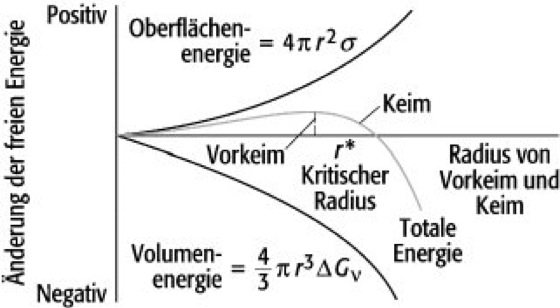
\includegraphics[width= 0.5 \linewidth]{img/radius}
			\caption{
			Darstellung der Änderung der freien Enthalpie in Abhängigkeit von der Keimgröße.
			Es ist leicht zu erkennen, dass ein kritischer Radius überschritten werden muss, damit der Keim stabil ist und wachsen kann.
			\cite{radius_enthalpie}
			}
			\label{fig_radius_enthalpie}
	\end{figure}

	Daraus ergibt sich, wie in \cref{fig_radius_enthalpie} zu erkennen ist, ein kritischer Radius, unter dem Keime nicht stabil sind und keine Kristallisation stattfinden kann.
	Dies ist darin begründet, dass die Grenzfläche zwischen kristalliner und amorpher Phase energetisch ungünstiger als beide Phasen ist.
	Da das Volumen mit $r^3$ und die Oberfläche mit $r^2$ geht, ist eine Erhöhung des Keimradiusses also erst ab einem bestimmten Radius energetisch günstig.

	Aus diesen Erkenntnissen folgt, dass bei der Frage, ob eine Abkühlende Schmelze kristallisiert, die Geschwindigkeit des Entstehens und Größe der Keime sowie die Geschwindigkeit des Abkühlens relevant sind.
	Wenn die Schmelze schnell genug abgekühlt wird bzw. die Probe ausreichend rein ist, können sich keine ausreichend große Keime bilden und sie erstarrt in amorpher Form (vgl. \cref{fig_kristallisierung}).

	\begin{figure}[H]
			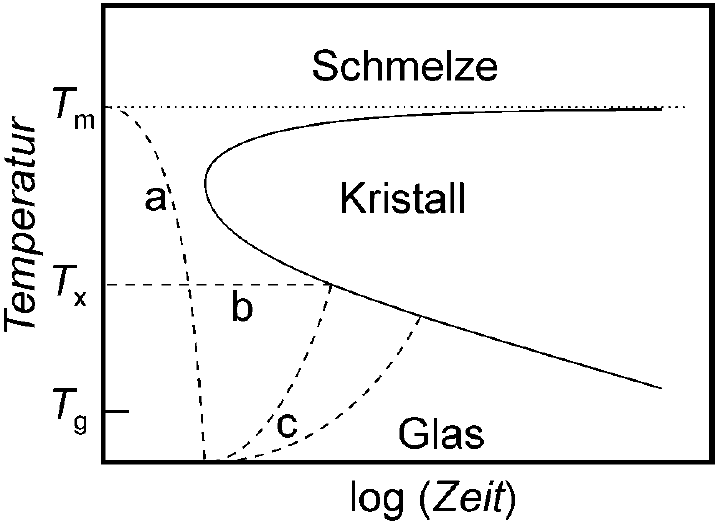
\includegraphics[width= 0.7 \linewidth]{img/kristallisierung}
			\caption{
			ZTU-Diagramm zu Kristallisation und Glasbildung
			a) schnelles Abschrecken
			b) isotherme Kristallisation
			c) Kristallisation für schnelle (links) und langsame (rechts) Aufheizrate
			\cite{anleitung}
			}
			\label{fig_kristallisierung}
	\end{figure}

	In \cref{fig_kristallisierung} ist als c) auch der umgekehrte Prozess dargestellt, welcher in diesem Versuch untersucht wird.
	Das Erhitzen eines Metalls in Glasphase führt dazu, dass es in den Bereich der unterkühlten Schmelze gerät, in der der oben beschriebene Keimbildungsprozess zur Kristallisation führen kann.
	Je schneller das Erhitzen stattfindet, desto eher kristallisiert das Glas, aber auch ein geringes Erhitzen gefolgt von einem Konstanthalten der Temperatur führt nach ausreichender Zeit zu Kristallisation.
	Demnach ist auch die zur Kristallisation zuzuführende Wärme (Kristallisationsenthalpie) abhängig von der Heizrate.
	Dieser Prozess ist irreversibel, weshalb ein Senken der Temperatur nicht wieder in die Glasphase führt.
	Hierfür wäre ein Schmelzen gefolgt vom oben geschilderte Prozess der schnellen Abkühlung erforderlich.

	Die Schmelzenthalpie eines Metalls ist demhingegen nur materialabhängig und kann mit Literaturwerten verglichen werden, da der Übergang von Schmelze zu Kristall reversibel ist.
	Hier ist also zu erwarten, dass die Schmelzenthalpie der Kristallisationsenthalpie entspricht. %TODO ist doch so, oder?

	\subsection{Röntgendiffraktometrie}
	Da ein amorpher Festkörper lediglich eine Nahordnung der Atome besitzen kann, während ein Kristall eine regelmäßige Gitterstruktur aufweist, ist zu erwarten, dass sich der amorphe Festkörper unter monochromatischem Röntgenlicht eher wie ein pulverisierter Kristall verhält und sich ein kontinuierliches Spektrum zeigt.
	Beim Kristall hingegen sind nur einige scharfe Reflexe zu erwarten, bei denen die Bragg-Gleichung erfüllt ist. %TODO nenne ich jetzt hier nicht, weil später?
	Aus der Position des Maximums beim amorphen Kristall lässt sich gemäß der Bragg-Gleichung der Mittlere Atomabstand berechnen.


	%\subsection{Vickers-Härte} %TODO ist schon weitgehend in Methoden

	\section{Methoden} %TODO Ziele angeben
	% Bilder von der Website klauen
	% einer will Präsens
	Es sollen drei verschiedene Untersuchungen bezüglich des Verhaltens von metallischen Gläsern durchgeführt werden.
	Hierzu wird als Vertreter der metallischen Gläser PdNiP verwendet.

	\subsection{Kalorimetrie}
	Es wird ein Leistungskalorimeter eingesetzt, um den Wärmefluss beim Erhitzen von verschiedenen Stoffen zu untersuchen.
	Zunächst wird eine Bleiprobe, die sich bereits in einem Tiegel befindet, im Vergleich zu einem Referenztiegel untersucht.
	Bei dieser wird keine gläserne Phase erwartet, da dies ein Erhitzen über den Schmelzpunkt gefolgt von einem schnelleren Abkühlen, als es mit diesem oder einem anderen bekannten Aufbau möglich ist, erfordern würde.
	Es werden zwei aufeinanderfolgende Messzyklen durchgeführt und das auf der Probe angegebene Gewicht notiert.

	Dann werden von einem Band aus amorphem PdNiP drei ungefähr gleich große Stücke mit einer Zange abgekniffen, gewogen und in Tiegeln verschlossen.
	Diese werden im Vergleich zu einem leeren Referenztiegel im Kalorimeter bei je unterschiedlicher Heizrate untersucht.
	Auch hier werden zwei Messzyklen aufgenommen.

	\subsection{Röntgendiffraktometrie} %lul steht in der Anleitung mindestens einmal falsch geschrieben
	In einem Röntgendiffraktometer (Kupfer-Anode, $\text{K}_\alpha$-Linie) wird im Debye-Scherrer-Verfahren die Röngenbeugung in Abhängigkeit vom Einstrahlwinkel unter monochromatischer Röntgenstrahlung gemessen.
	Dabei wird eine amorphe und eine kristalline PdNiP-Probe untersucht.
	Beiden werden nicht pulverisiert.	%TODO weil pulver erwartung, dass bei kristall nichts exaktes

	\subsection{Messung der Vickershärte}
 	Es wird ein Mikroindenter verwendet, um die Vickershärte einer Probe aus kristallinem und einer aus amorphem PdNiP zu bestimmen. %TODO das steht in der Anleitung, aber an den Daten steht was von Paradin-Phosphor (was nicht existiert) und Ni.
	Dazu wird ein Diamant in Form einer vierseitigen Pyramide mit einem Öffnungswinkel von \SI{136}{\degree} für \SI{5}{s} mit einer Kraft von \SI{0.5}{kgf} auf die Probe gedrückt.
	Dann wird mit einem Mikroskop die Länge der beiden Diagonalen gemessen.
	Das verwendete Gerät errechnet dann aus diesen Werten die Vickershärte.
	Es werden jeweils \num{10} Messungen durchgeführt, um einen Mittelwert bilden zu können.

	\section{Ergebnisse und Diskussion}
	%TODO Unsicherheiten

	\subsection{Kalorimetrie}
	\subsubsection{Unsicherheiten}
	\subsubsection{Beobachtung und Datenanalyse}
	\subsubsection{Diskussion}
	%TODO Schmelzenthalpie mit Lit. vergleichen
	%TODO Kristallisationsenthalpie ist abhängig von Heizrate/Unterkühlung
	%TODO Übersteuerung am Ende durch Umschalten von Heizen zu Kühlen.
	Der Literaturwert der Schmelzenthalpie von Blei beträgt \SI{4,8}{\kilo \joule \per \mol} \cite{blei_enthalpie}.
	%TODO Blei: Nur schmelzen/kristallisation -> reversibel und Schmelz=Kristallisation
	%TODO PdNiP: irreversibel-> keine Erneute Kristallisation
	%TODO zwei Peaks, weil vmtl im MAterial Bereiche mit PdNi und welche mit NiP, sodass der eine Teil erst Kristallisiert.
	\subsection{Röntgendiffraktometrie}
	%\subsubsection{Unsicherheiten} %hab ich bissle im Beob diskutiert.
	\subsubsection{Beobachtung und Datenanalyse}
	Die gemessenen Kurven sind in \cref{fig_xrd_kristallin} und \cref{fig_xrd_glas} dargestellt.
	Bei $\theta \approx \SI{31}{\degree}$ ist in der Messung der kristallinen Probe eine deutliche Kante zuerkennen.
	Sie kennzeichnet den Punkt an dem die Probe aus der Halterung gefallen ist und somit keine sinnvolle Messung mehr möglich war.
	Aus dem Abschnitt ohne Probe lässt sich gut eine Unsicherheit und der Untergrund abschätzen, da man ohne eine Probe keine Ereignisse erwartet. %TODO ist irgendwie nicht "gut", wenn man danach sagt, dass es nicht gut ist.
	Jedoch ist die Schwankung während der Messung deutlich größer als die so abgeschätze Unsicherheit, weshalb diese vernachlässigt wird.
	\begin{figure}[H]
			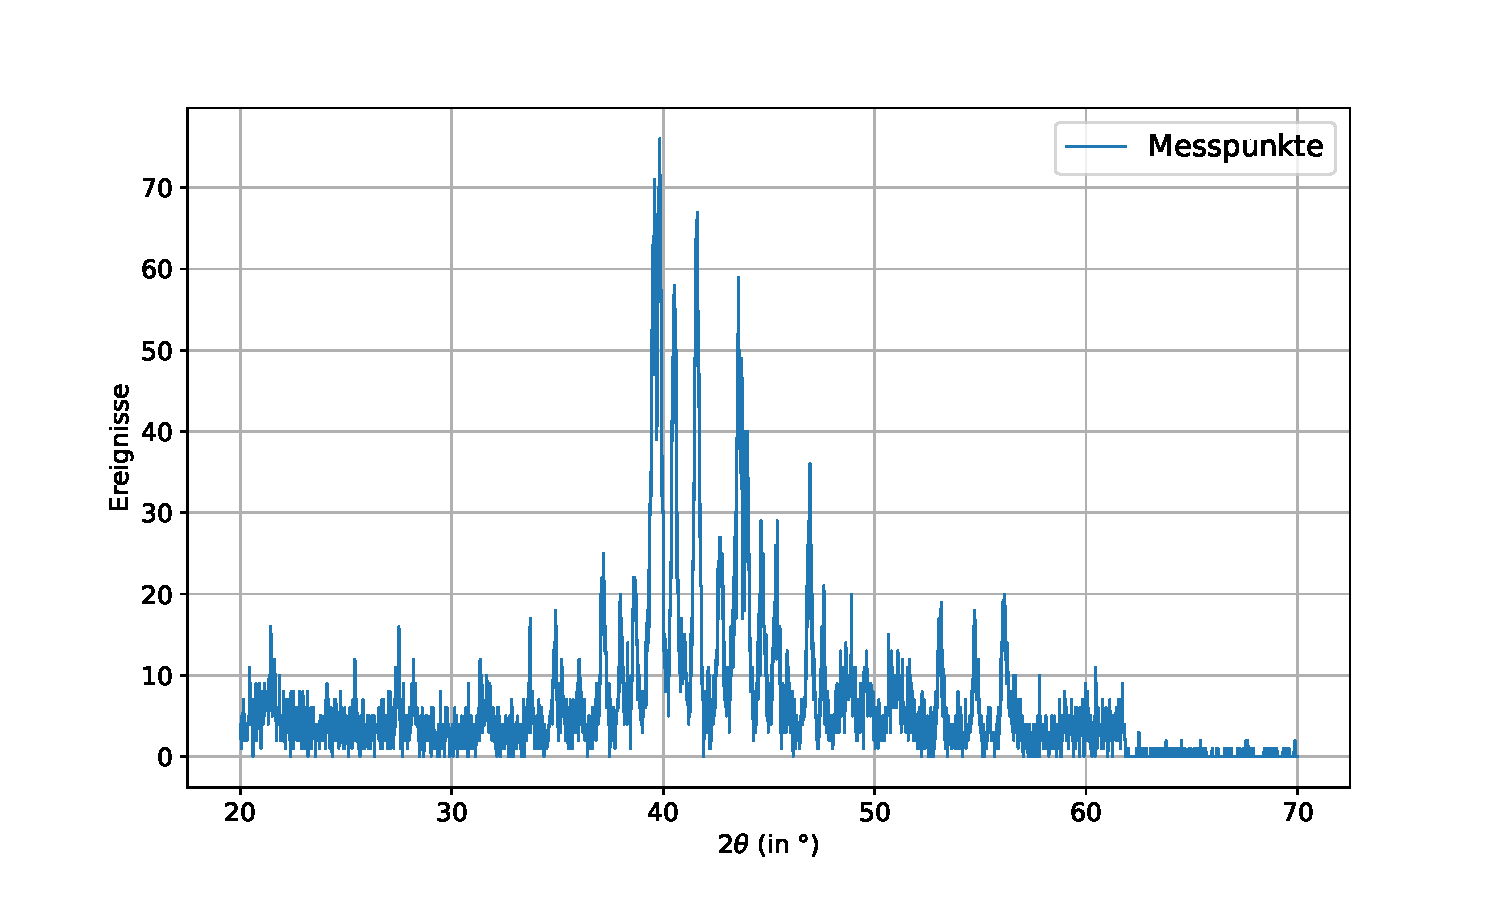
\includegraphics[width=\linewidth]{img/XRD_Kristallin_45_25.pdf}
			\caption{Diffraktogramm der kristallinen Probe.}
			\label{fig_xrd_kristallin}
	\end{figure}
	\begin{figure}[H]
			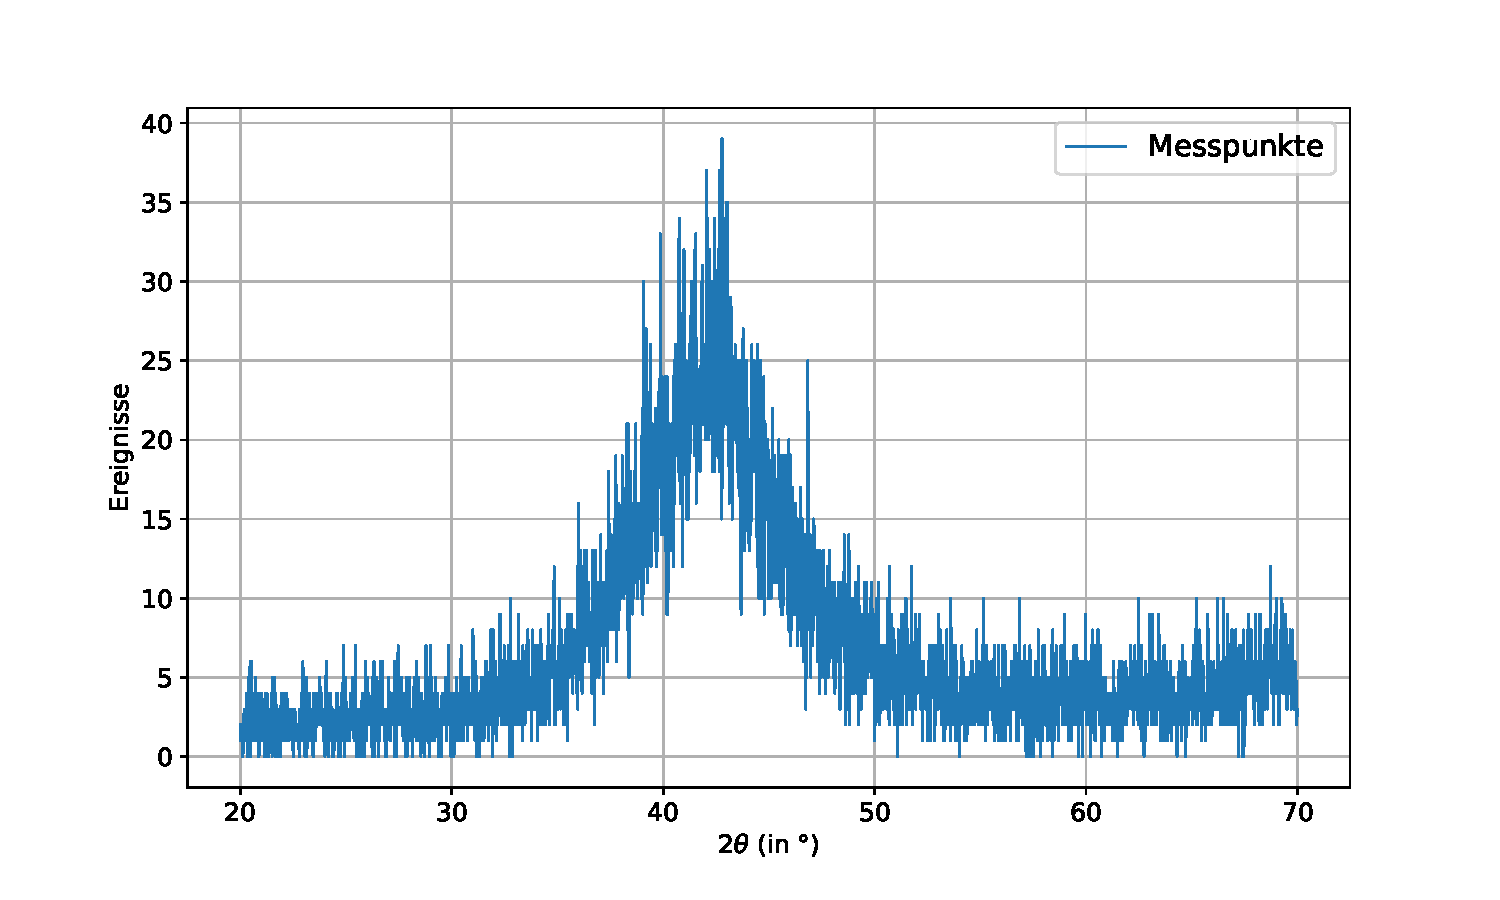
\includegraphics[width=\linewidth]{img/XRD_Glas_45_25.pdf}
			\caption{Diffraktogramm der Glasprobe.}
			\label{fig_xrd_glas}
	\end{figure}

	Zur Bestimmung der Positionen und Breiten der Peaks werden Gauß-Funktionen an die Messungen in einem Intervall um den Peak gefittet (vgl. \nameref{s_anhang}):
	\begin{equation}
		\label{eq_gauss}
		f(x) = a\cdot e^{-\frac{(x - c)^2}{2d^2}} + y
	\end{equation}
	Die gemittelten Peakpositionen der Proben befinden sich in \cref{tb_xrd_result}.
	Außerdem wurde nach der Bragg-\cref{eq_bragg} der Abstand der Gitterebenen, bzw. der mittler Atomabstand berechnet.
	\begin{equation}
			\label{eq_bragg}
			\bar{d} = \frac{\lambda}{2\sin{\bar{\theta}}} \quad \text{mit} \quad u(\bar{d}) = \left|\frac{\cos{\bar{\theta}}}{2\sin^2{\bar{\theta}}} \right| \lambda \cdot u(\bar{\theta})
	\end{equation}
	Die Wellenlänge der Röntgenstrahlung einer Kupfer-Anode beträgt $\lambda_{\text{K}_\alpha}= \SI{1.5406}{\angstrom}$.
	\begin{table}[H] %TODO die haut sich rechts raus.
		\centering
		\begin{tabular}{ c | c | c | c | c | c}
			 Probe& Glas  &\multicolumn{4}{c}{Kristall} \\ \hline
			 Peak&  1 & 1 & 2 &  3 & 4\\ \hline
			 $2\bar{\theta}$&\SI{42.2+-1.3}{\degree}&\SI{39.7+-0.3}{\degree} & \SI{40.52+-0.19}{\degree} &\SI{41.59+-0.16}{\degree} & \SI{43.6+-0.43}{\degree} \\
			 $\bar{d}$ &\SI{2.14+-0.06}{\angstrom} & \SI{2.27+-0.02}{\angstrom} & \SI{2.224+-0.010}{\angstrom} & \SI{2.17+-0.008}{\angstrom} & \SI{2.07+-0.02}{\angstrom}
		\end{tabular}
		\caption{Positionen der Diffraktogramm Peaks, sowie die aus der Bragg-\cref{eq_bragg} resultierenden Gitterebenenabstände (Kristall), bzw. der mittlere Atomabstand (Glas).}
		\label{tb_xrd_result}
\end{table}
	\subsubsection{Diskussion}
	%TODO anleitung sagt 3 maximalsten peaks, würde ich dann halt die schöneren 3 der 4 nehmen, oder alle weil ca. gleich hoch
	Rein qualitativ lässt sich sofort feststellen, dass erwartungsgemäß das Spektrum vom metallischen Glas in \cref{fig_xrd_glas} kontinuierlich ist, während das des Kristalls in \cref{fig_xrd_kristallin} eher diskret ist, was dafür spricht, dass die Glasprobe tatsächlich amorph ist. %TODO zu vorsichtig?
	\cite{SIETSMA1991146} gibt die Atomabstände in \cref{tb_xrd_vgl} aus einer Kombination aus theoretischer Berechnung mit radialen Verteilungsfunktionen und experimenteller Bestimmung.
	Sie lassen sich nicht eindeutig den Messwerten in \cref{tb_xrd_result} zuordnen, da in der durchgeführten Messung nicht zwischen Atomsorten unterschieden werden kann. Der Messwert liegt aber zwischen den Literaturwerten für die einzelnen Atome, weshalb hier kein Widerspruch gezeigt werden kann. %TODO komisch vormuliert, ab idk

	\begin{table}[H]
		\centering
		\begin{tabular}{ c | c | c | c }%TODO die haut sich rechts raus.
			 Peak&  $\sigma_1$ & $\sigma_2$ & $\sigma_3$\\ \hline
			  & Pd \SI{2.8}{\angstrom} & Ni \SI{2.4}{\angstrom} & P \SI{1.8}{\angstrom}
		\end{tabular}
		\caption{Die in \cite{SIETSMA1991146} für Glas (PdNiP) angegebenen Atomdurchmesser. Sie wurden dort als beste Übereinstimmung von Experiment und Berechnung gewählt. Da mit Atomdurchmesser hier der Platz gemeint ist, den das Atom im Gitter einnimmt, ist er hier als mittlerer Atomabstand zu verstehen. Die Unsicherheit beträgt etwa \SI{0.005}{\angstrom}.} %TODO das ist bissl riskant, weil ich nicht 100% sicher bin, ob das true ist.
		\label{tb_xrd_vgl}
\end{table}

	%TODO ich finde keinen Literaturwert für PdNiP in kristallförmig.
	%Die Größe der Schwankungen könnte dadurch zustande kommen, dass
	%TODO Absorption? naja. Drehprozess? Ist der ruckartig? misst der dazwischen?
	%TODO warum sind die Schwankungen so riesig?

	\subsection{Messung der Vickershärte}
	\subsubsection{Unsicherheiten} \label{sss_vicker_unsicher}
	Die Vickershärte wird direkt am Mikroskop von einer Digitalanzeige abgelesen.
	Mit einer Rechteckverteilung ergibt sich eine Unsicherheit von $u(H) = \SI{0.03}{HV}$.
	\subsubsection{Beobachtung und Datenanalyse}
	%TODO mehr Text hier
	In \cref{fig_indents} sind beispielhafte Aufnahmen des Mikroskops dargestellt.
	\begin{figure}[H]
		\centering
			\subcaptionbox{
				PdNiP-Probe.\label{fig_indent_pdnip}}{
			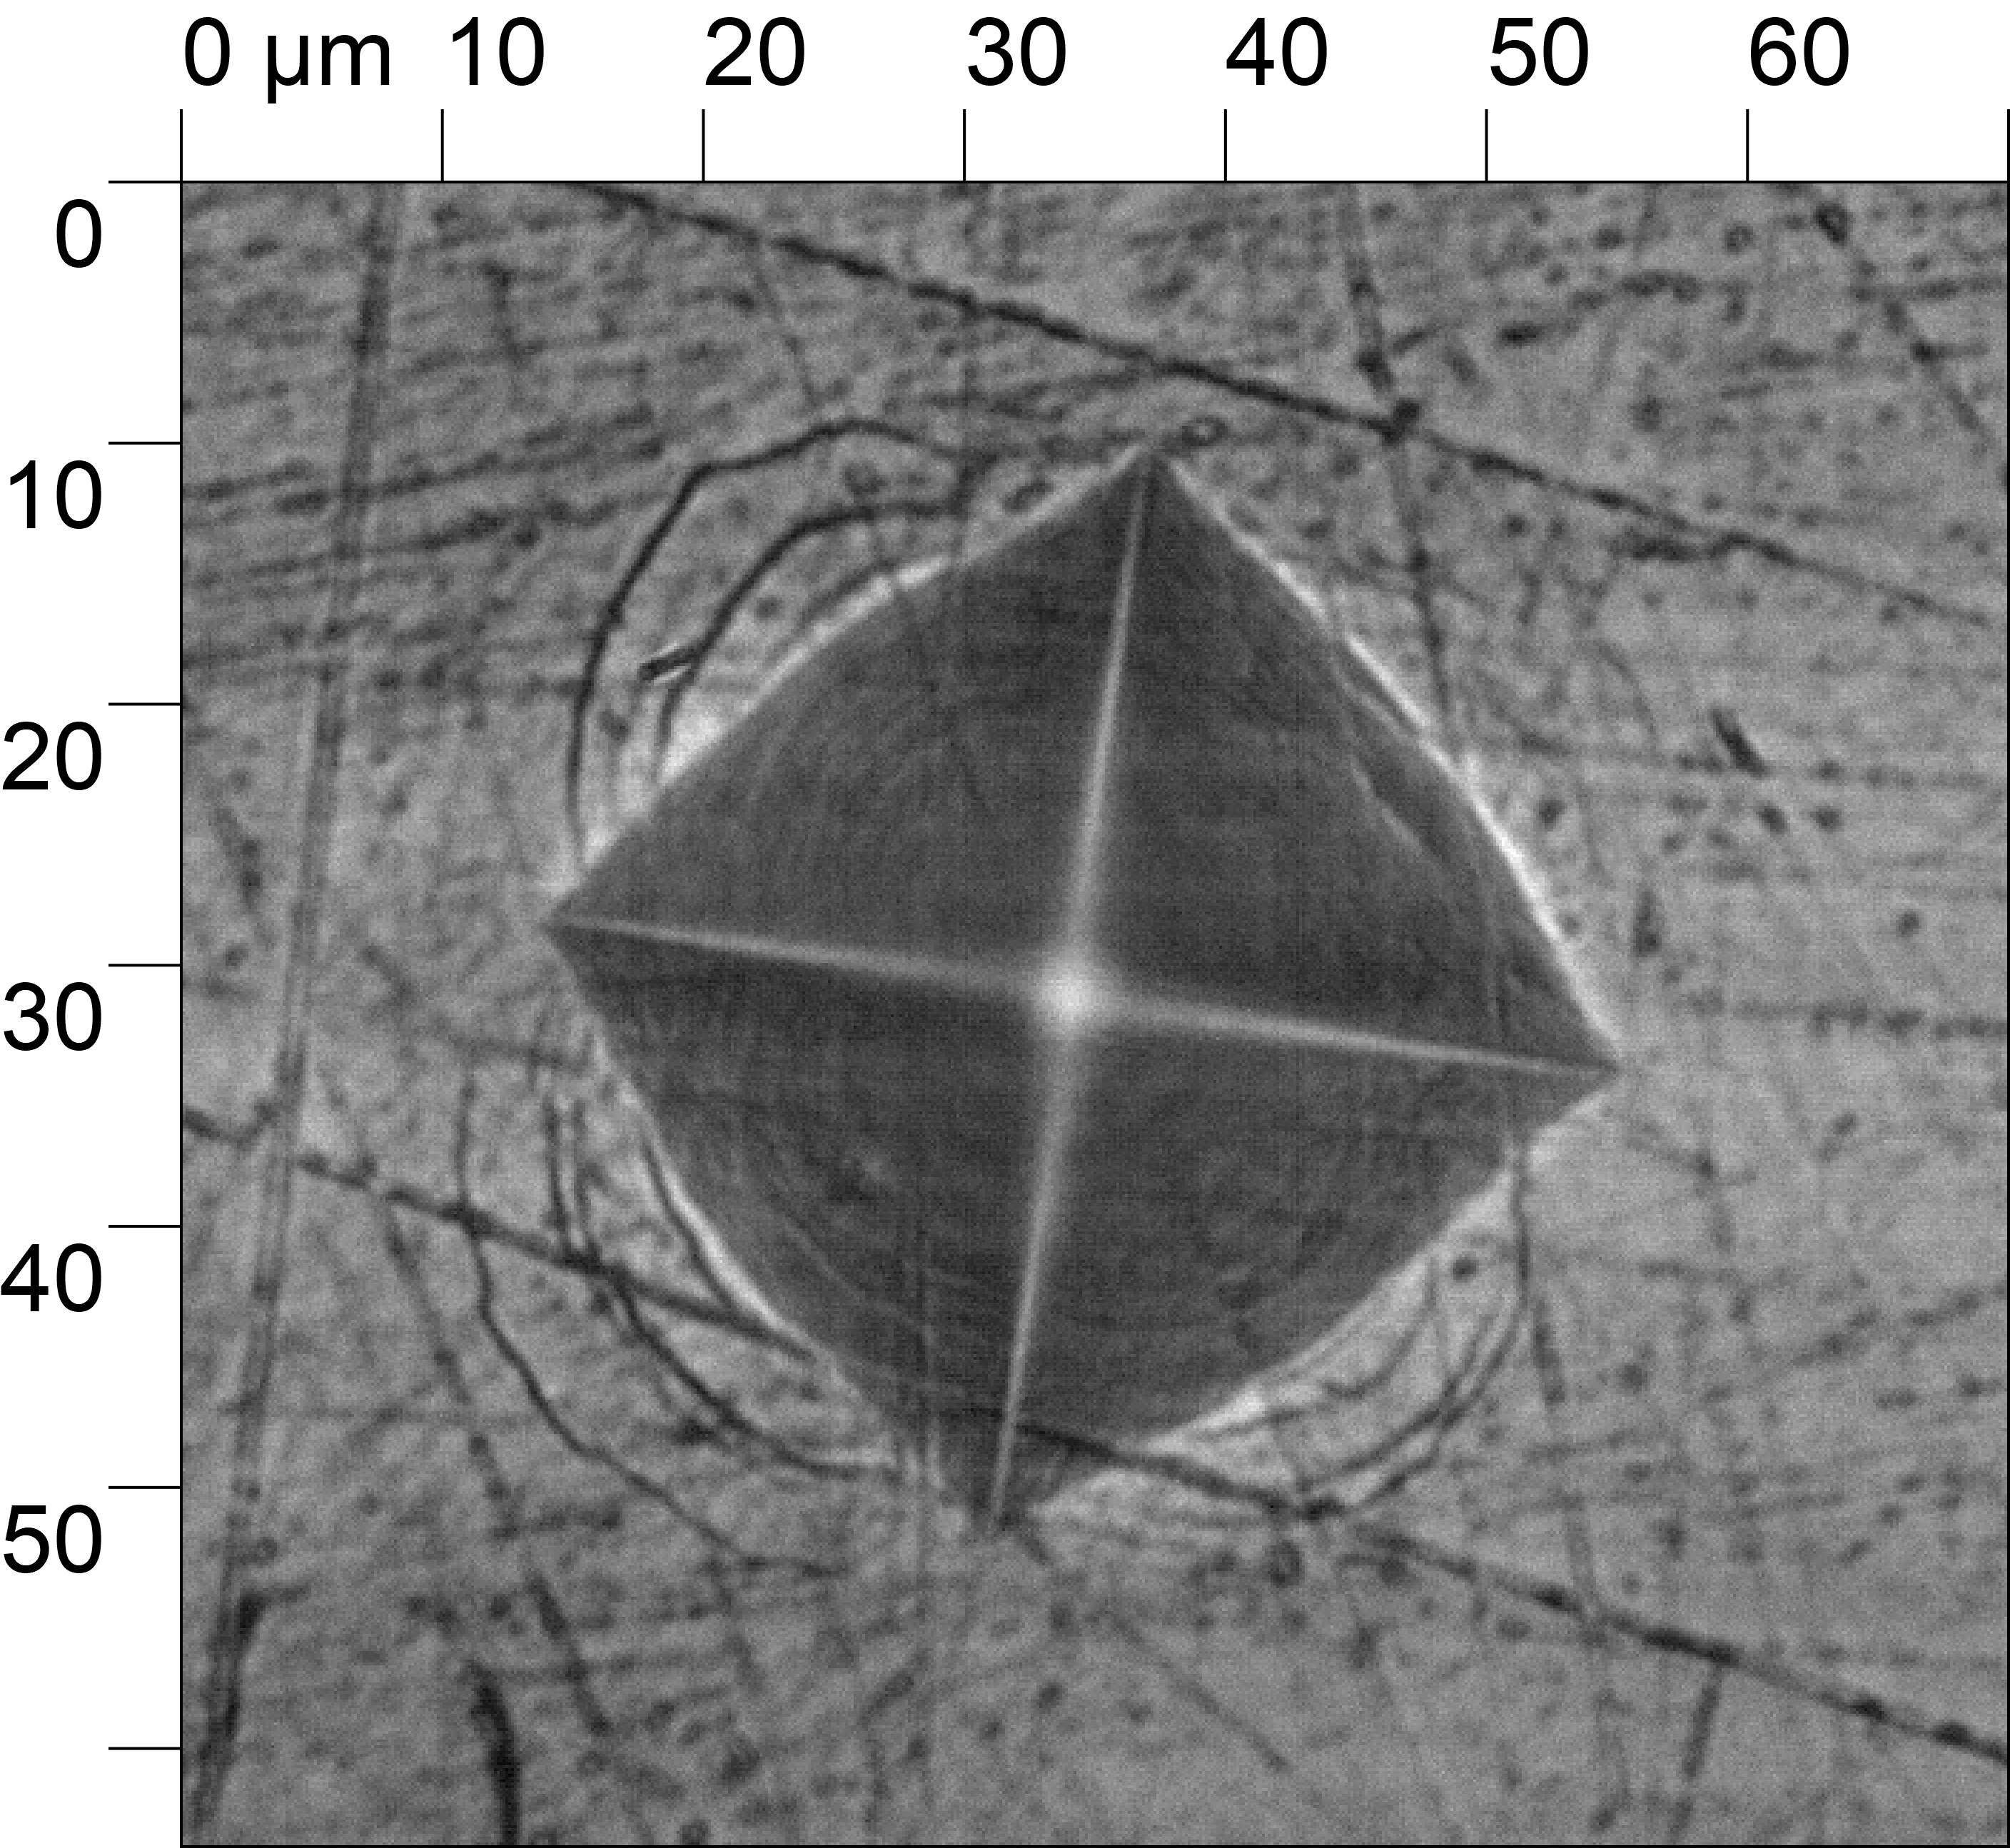
\includegraphics[width=.47\linewidth]{img/Paradin-Phosphor-500N-5s-l}}
			\subcaptionbox{
				Nickel-Probe.\label{fig_indent_ni}}{
			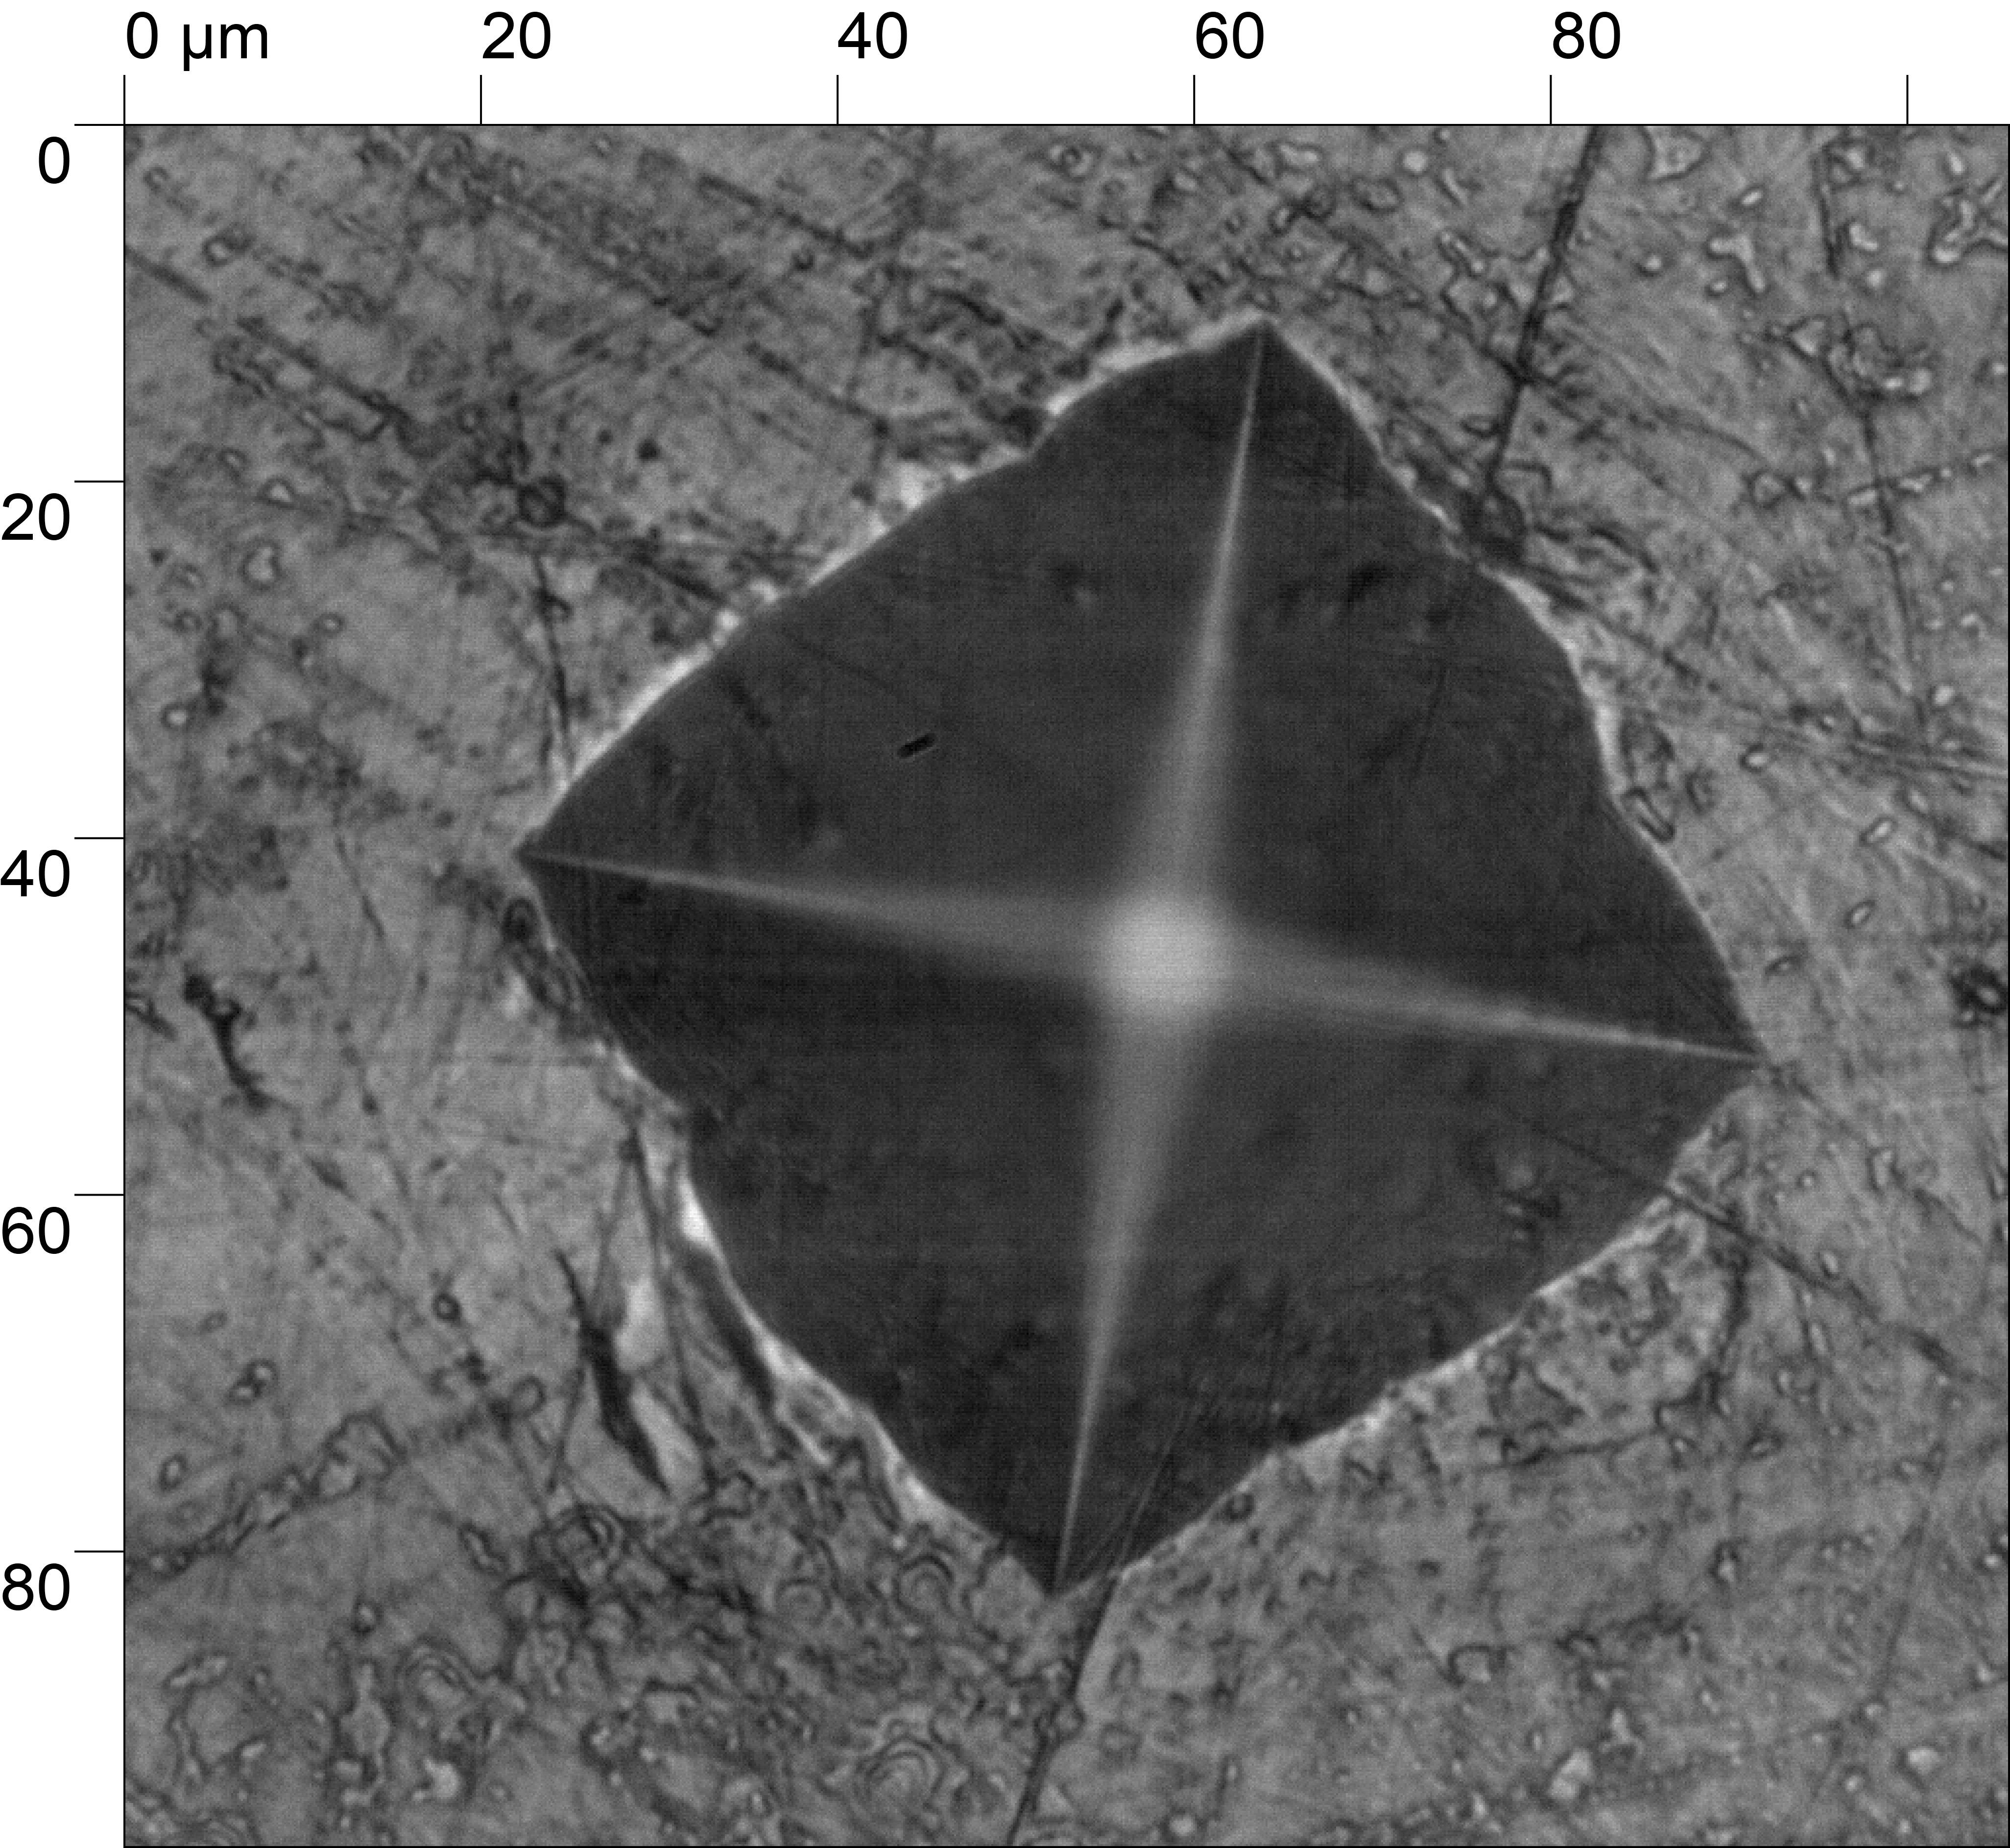
\includegraphics[width=.47\linewidth]{img/Ni-500N-5s-l}}
			\caption{Abdrücke der Indenterpyramide auf verschiedenen Proben. Der Fokus ist auf die Probenebene gelegt, weshalb die Mitte des Abdrucks unscharf ist.}
			\label{fig_indents}
 \end{figure}
 Der Mittelwert $\bar{H}$ von N Messungen berechnet sich nach GUM wie folgt:
 \begin{equation}
	 \bar{H} = \frac{1}{N}\sum_{i=1}^N H_i \quad \text{mit} \quad u(\bar{H}) = \sqrt{\sum_{i=1}^N \frac{(H_i-\bar{H})^2}{N-1}}
 \end{equation}
 Die gemittelte Vickershärte der Nickel-Probe beträgt \SI{188+-5}{HV} und die der PdNiP-Probe \SI{534+-14}{HV}.
 Die Unsicherheit durch die Digitalanzeige (vgl. \ref{sss_vicker_unsicher}) verschwindet gegenüber der Standardabweichung der Mittelwerte.

	\subsubsection{Diskussion}
	% Bilder vergleichen, dass erwähnen was er meinte mit man sieht schön die 'Brechung'/'Verschiebung' oder so, kp was es war
	% wie erwartet Glas härter

	In \cref{fig_indents} ist zu erkennen, dass bei der PdNiP-Probe dauerhafte Verformungen außerhalb des Pyramidenabdrucks auftreten.
	In der Nickel-Probe ist das nicht der Fall.
	Dies liegt daran, dass im Kristall bei einer Verformung die geschobenen Atome einfach einige Gitterpositionen weiter springen können, ohne die Gitterstruktur zu verletzen.
	Im amorphen PdNiP ist dies nicht möglich, weshalb Bereiche anderer Nahordnung ebenfalls geschoben werden und die beobachteten \enquote{ripples} auftreten. %TODO ripple fine?
	Diese leichtere Verschiebbarkeit der Atome im Kristall im Vergleich zum amorphem Glas ist auch der Grund dafür, dass die PdNiP-Probe die beobachtete deutlich höhere Vickers-Härte (\SI{524 \pm 14}{HV}) als die kristalline Nickel-Probe (\SI{188 \pm 5}{HV}) hat.
	%TODO Notes für Diskussion v , weil abgetrennt >>???
	% Bezug/Nutzen oder sonst was
	% auch hier die Hypothese wiederholen
	% keine Messwerte hier, nach manchen Menschen, zumindest "direkt" erstellte Diagramme net hier, auch wenn Lesbarkeit-bla

	\section{Schlussfolgerung}
	% Rückgriff auf Hypothese und drittes Nennen dieser

	% Quellen zitieren, Websiten mit Zugriffsdatum
	% Verweise auf das Laborbuch (sind erlaubt)
	% Tabelle + Bilder mit Beschriftung
	\printbibliography



	\section{Anhang} \label{s_anhang}
	%TODO image sizes/scaling 2 Bilder auf 1 Seite?
	\subsection{Röntgendiffraktometrie}

	\begin{figure}[H]
			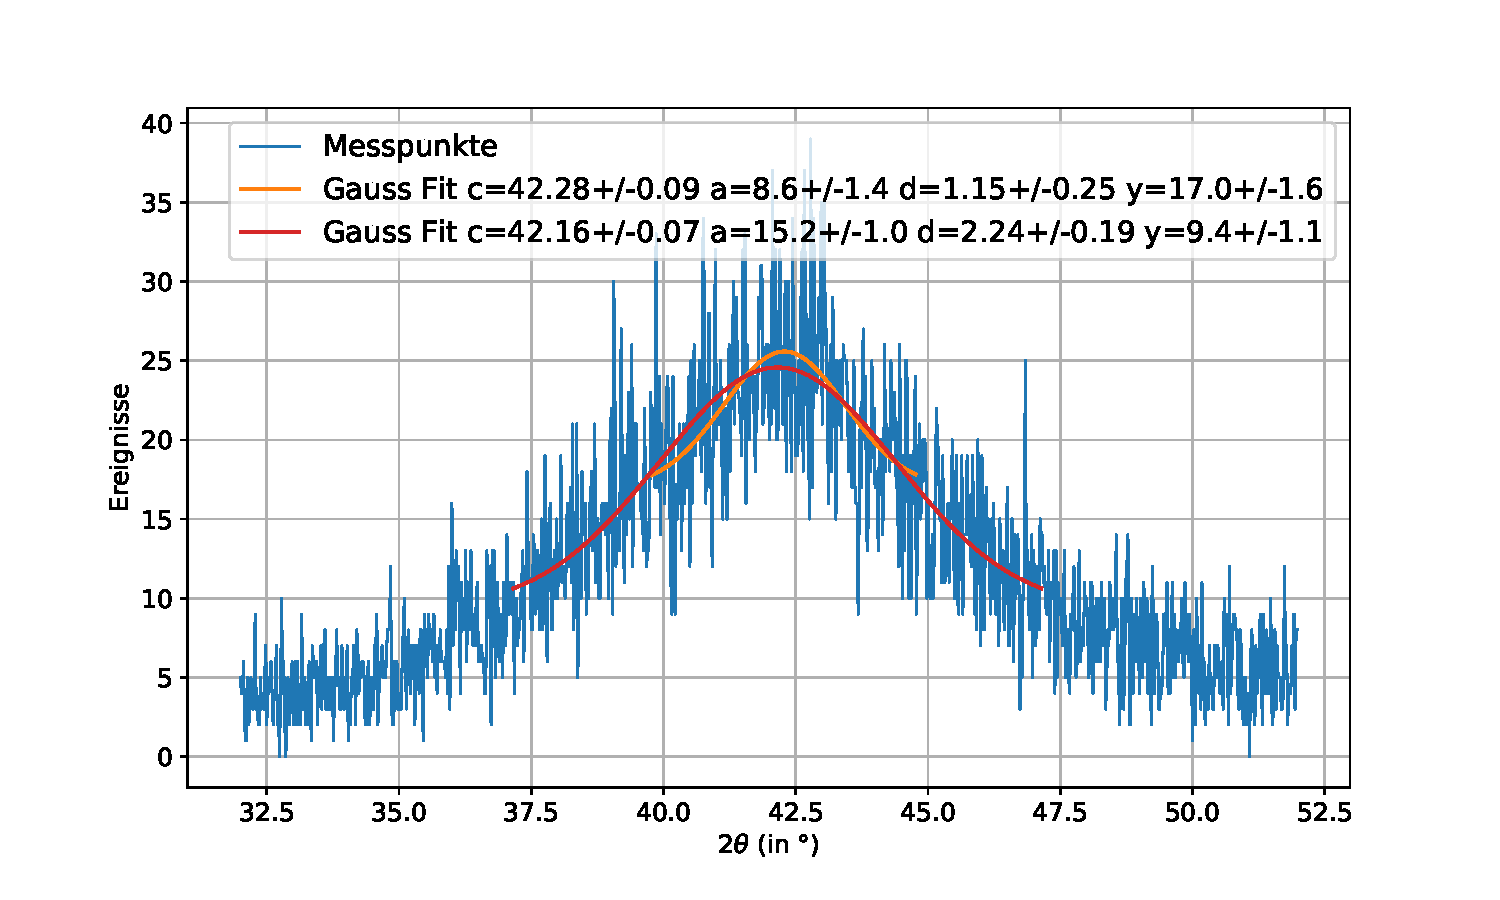
\includegraphics[width=\linewidth]{img/XRD_Glas_42_10.pdf}
			\caption{
				Vergrößertes Diffraktogramm der Glasprobe.
				Die Fitfunktionen sind Gauß-Funktionen nach \cref{eq_gauss}.
				Die für den Fit einbezogenen Messpunkte entstammen dem Intervall, in welchem die jeweilige Gauß-Funktion abgebildet ist.
				}
			\label{fig_xrd_glas_1}
	\end{figure}



	\begin{figure}[H]
			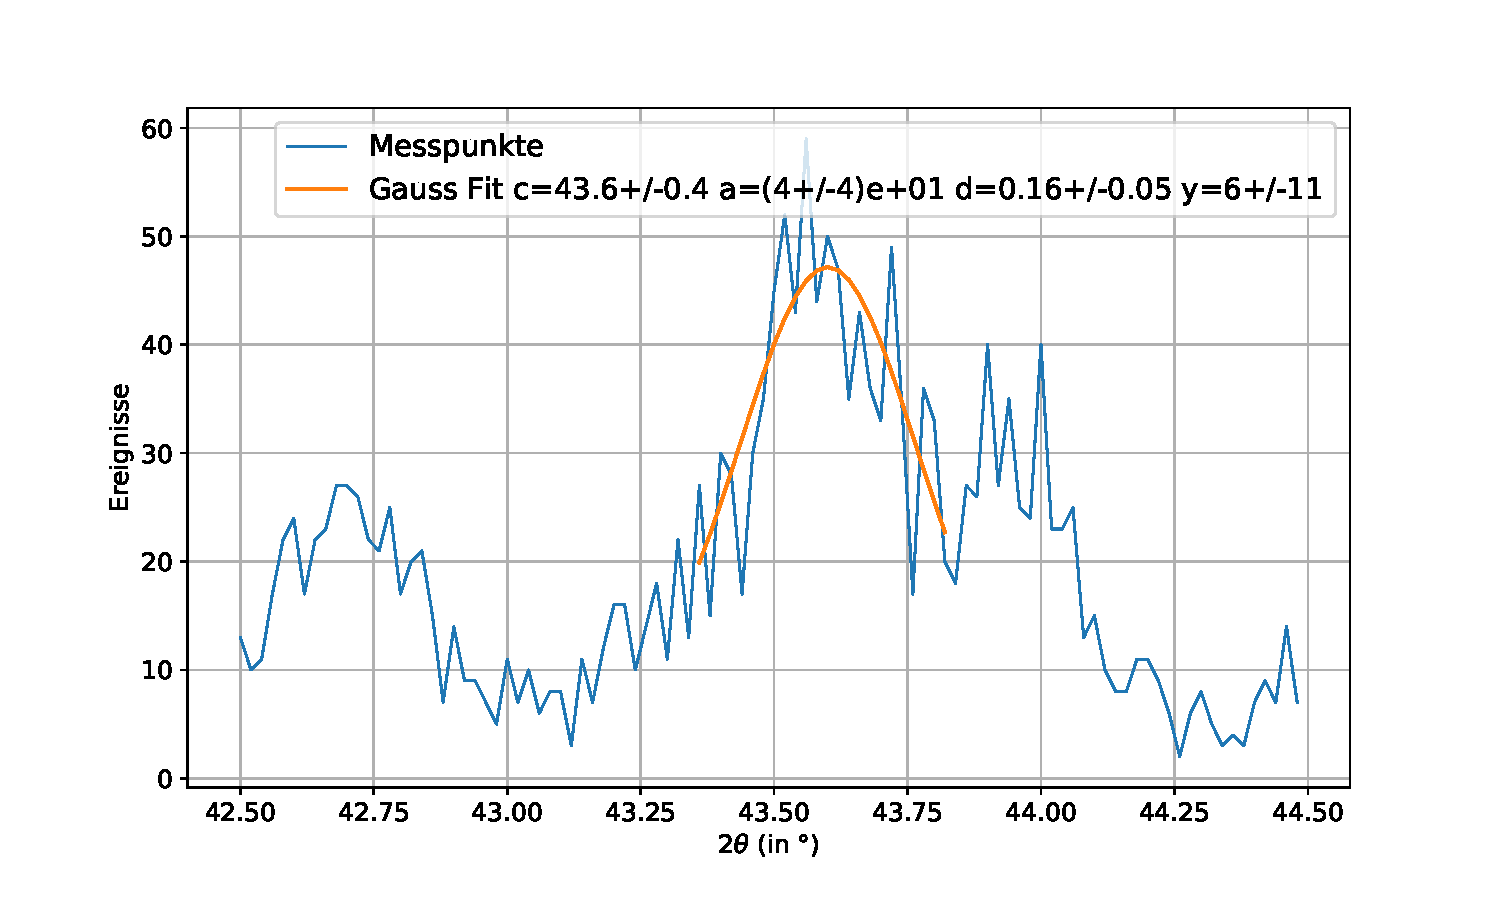
\includegraphics[width=\linewidth]{img/XRD_Kristallin_43,5_1.pdf}
			\caption{
				Vergrößertes Diffraktogramm der kristallinen Probe.
				Die Fitfunktionen sind Gauß-Funktionen nach \cref{eq_gauss}.
				Die für den Fit einbezogenen Messpunkte entstammen dem Intervall, in welchem die jeweilige Gauß-Funktion abgebildet ist.
				}
			\label{fig_xrd_kristall_1}
	\end{figure}
	\begin{figure}[H]
			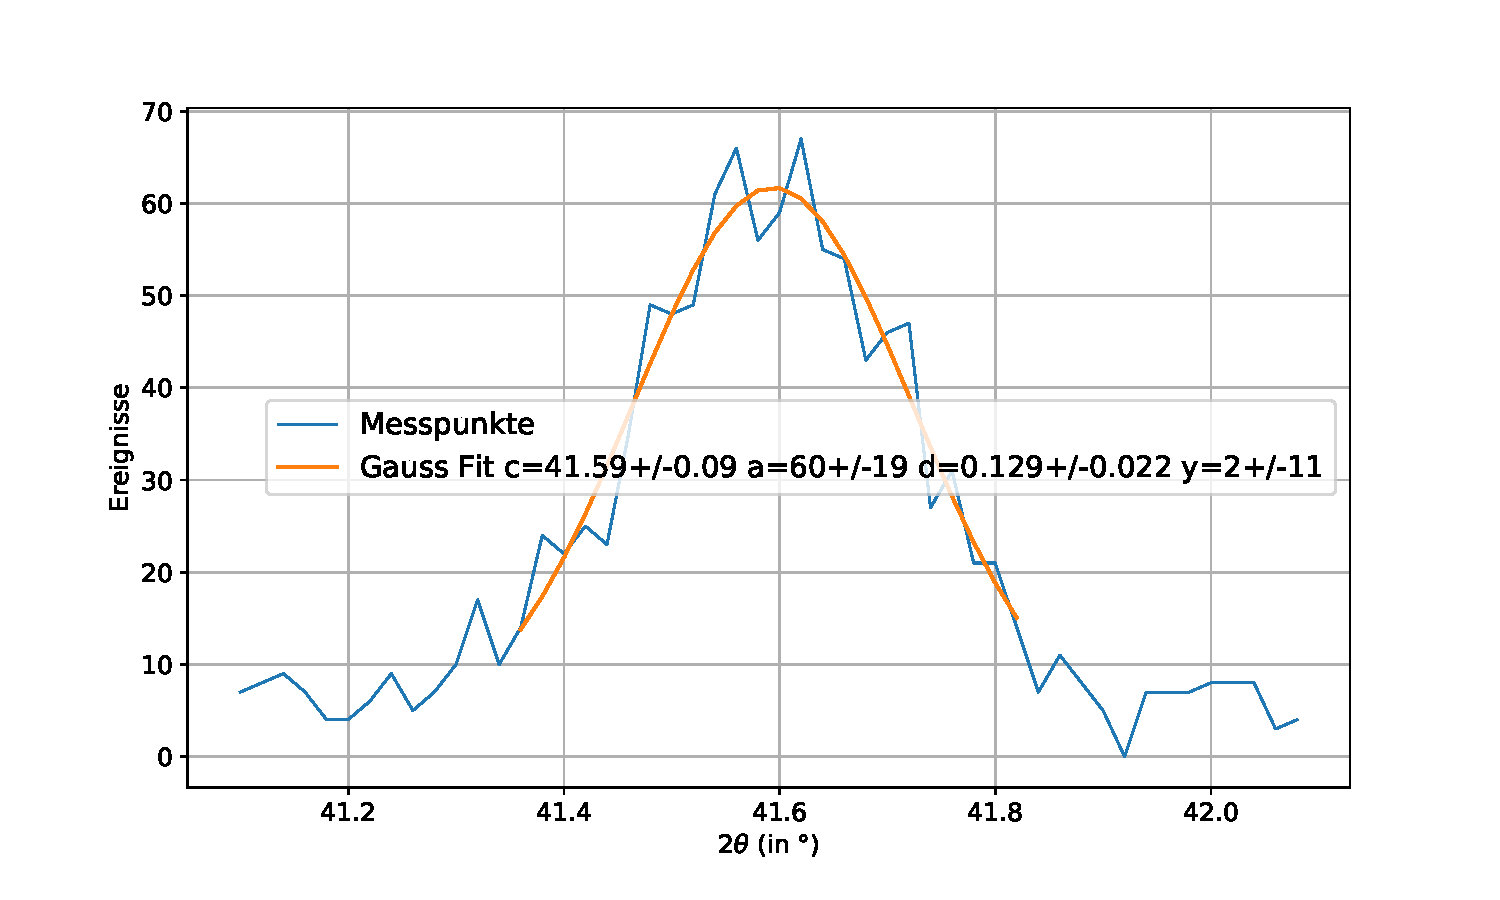
\includegraphics[width=\linewidth]{img/XRD_Kristallin_41,6_0,5.pdf}
			\caption{
				Vergrößertes Diffraktogramm der kristallinen Probe.
				Die Fitfunktionen sind Gauß-Funktionen nach \cref{eq_gauss}.
				Die für den Fit einbezogenen Messpunkte entstammen dem Intervall, in welchem die jeweilige Gauß-Funktion abgebildet ist.
				}
			\label{fig_xrd_kristall_2}
	\end{figure}
	\begin{figure}[H]
			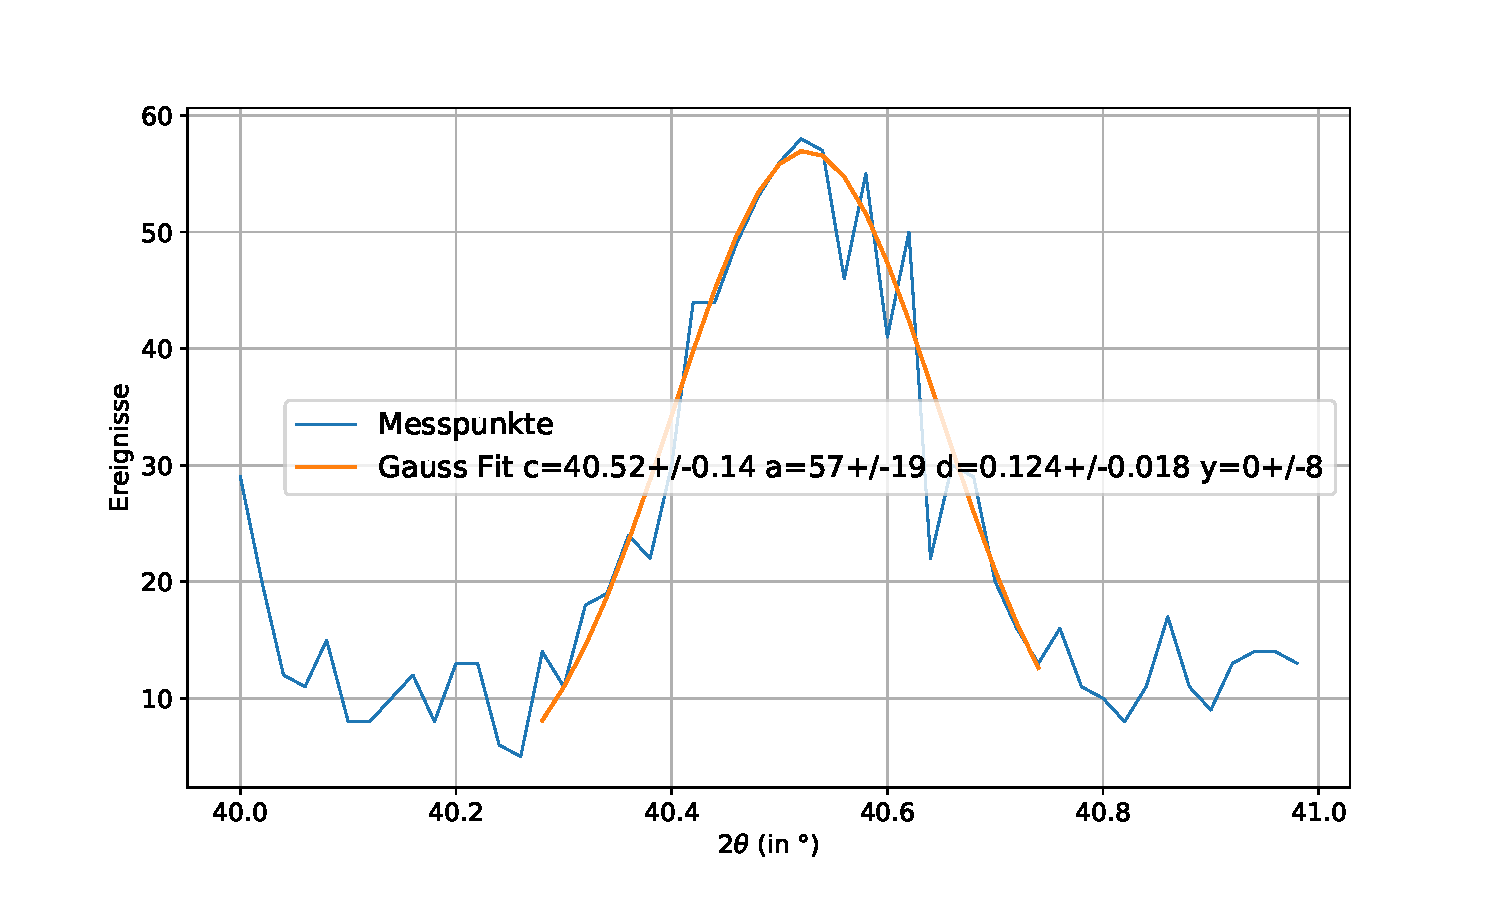
\includegraphics[width=\linewidth]{img/XRD_Kristallin_40,5_0,5.pdf}
			\caption{
				Vergrößertes Diffraktogramm der kristallinen Probe.
				Die Fitfunktionen sind Gauß-Funktionen nach \cref{eq_gauss}.
				Die für den Fit einbezogenen Messpunkte entstammen dem Intervall, in welchem die jeweilige Gauß-Funktion abgebildet ist.
				}
			\label{fig_xrd_kristall_3}
	\end{figure}
	\begin{figure}[H]
			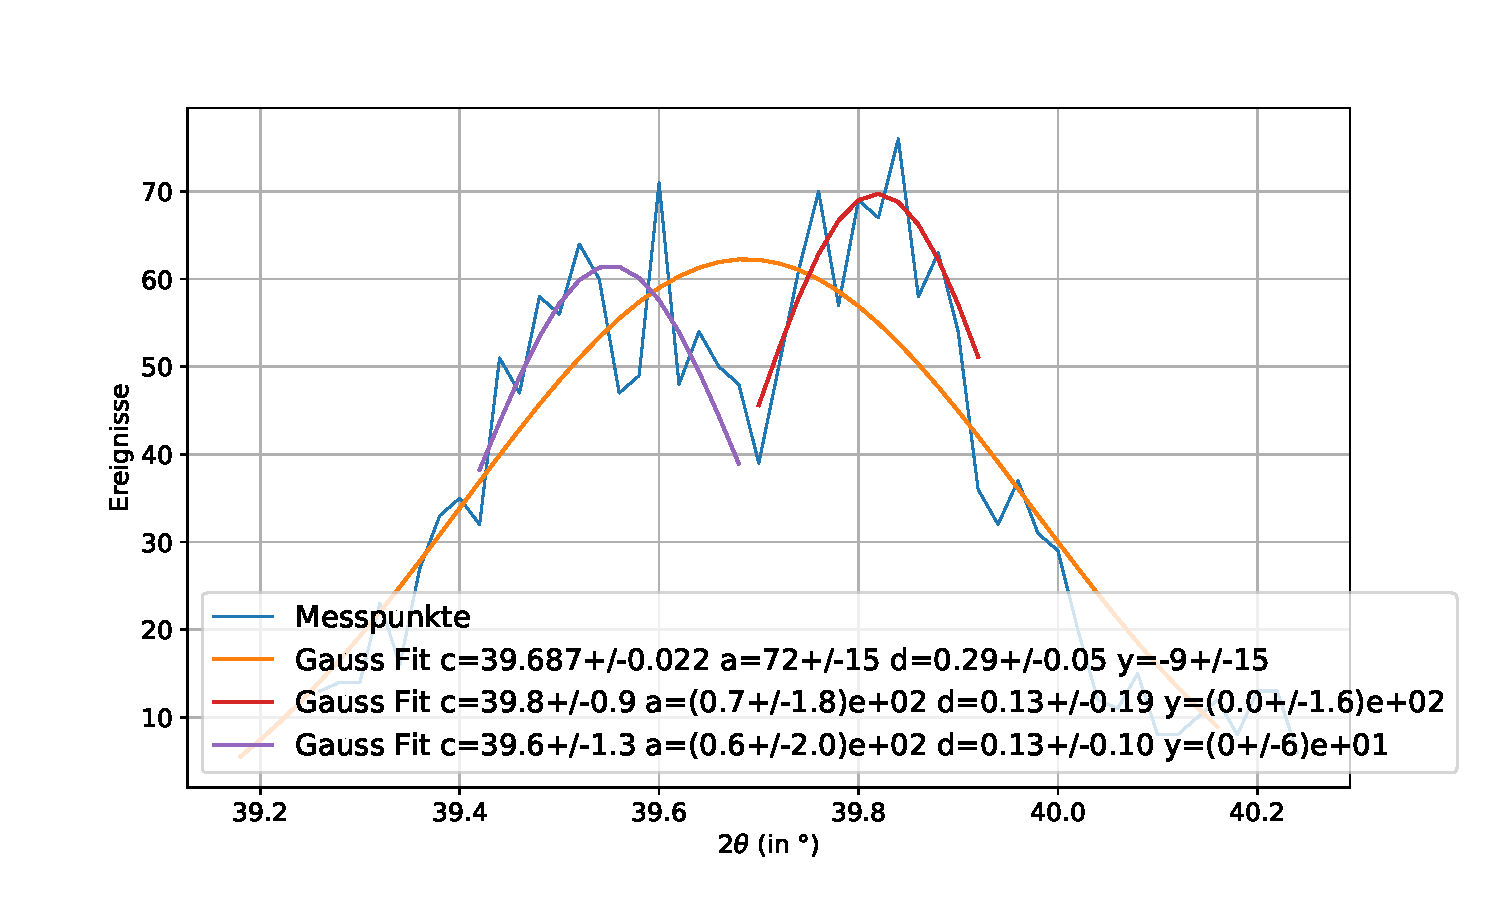
\includegraphics[width=\linewidth]{img/XRD_Kristallin_39,76_0,5.pdf}
			\caption{
				Vergrößertes Diffraktogramm der kristallinen Probe.
				Die Fitfunktionen sind Gauß-Funktionen nach \cref{eq_gauss}.
				Die für den Fit einbezogenen Messpunkte entstammen dem Intervall in welchem die jeweilige Gauß-Funktion abgebildet ist.
				}
			\label{fig_xrd_kristall_4}
	\end{figure}
\end{document}

%TODO Angleichen: Vickers-Härte/Vickershärte.
